\documentclass{tufte-handout}

\title{Road safety's Vision Zero: applications to OH\&S}

\author{Dr James Reynolds, Public Transport Research Group}

%\date{28 March 2010} % without \date command, current date is supplied

%\geometry{showframe} % display margins for debugging page layout

\usepackage{graphicx} % allow embedded images
  \setkeys{Gin}{width=\linewidth,totalheight=\textheight,keepaspectratio}
  \graphicspath{{graphics/}} % set of paths to search for images
\usepackage{amsmath}  % extended mathematics
\usepackage{booktabs} % book-quality tables
\usepackage{units}    % non-stacked fractions and better unit spacing
\usepackage{multicol} % multiple column layout facilities
\usepackage{lipsum}   % filler text
\usepackage{fancyvrb} % extended verbatim environments
\usepackage{pgfplots}
  \fvset{fontsize=\normalsize}% default font size for fancy-verbatim environments

% Standardize command font styles and environments
\newcommand{\doccmd}[1]{\texttt{\textbackslash#1}}% command name -- adds backslash automatically
\newcommand{\docopt}[1]{\ensuremath{\langle}\textrm{\textit{#1}}\ensuremath{\rangle}}% optional command argument
\newcommand{\docarg}[1]{\textrm{\textit{#1}}}% (required) command argument
\newcommand{\docenv}[1]{\textsf{#1}}% environment name
\newcommand{\docpkg}[1]{\texttt{#1}}% package name
\newcommand{\doccls}[1]{\texttt{#1}}% document class name
\newcommand{\docclsopt}[1]{\texttt{#1}}% document class option name
\newenvironment{docspec}{\begin{quote}\noindent}{\end{quote}}% command specification environment

\begin{document}

\maketitle% this prints the handout title, author, and date

\begin{abstract}
\noindent
Researchers across Monash, including from Civil Engineering and the Accident Research Centre (MUARC), have long been involved in road safety. This has included advocating for wider adoption of the Safe System approach\cite{TAC:2016aa}, in which there is an acknowledgement that human error is inevitable, and that it is road designers and managers, rather than users, who have primary responsibility for ensuring safe outcomes. Underlying this is 'Vision Zero': a philosophy that death or serious injury should never be the outcome of a road system failure\cite{Lydon:2017aa}.

Are our current  approaches to (non-road-related) OH\&S matters aligned with Safe System principles? This Safety Day discussion explores these issues, and provides perspectives from road safety engineering, where death and serious injury remains a daily occurrence, on how workplace safety management might be further improved.\end{abstract}

%A Road Safety Audit (RSA) is a formal process used in traffic engineering to assess the crash potential of new and existing facilities. The aim is to identify potentially hazardous conditions and recommendations.  It is often used during design or immediately after construction is complete so that unsafe features can be identified and corrected  \textbf{before} anyone uses the road. 


\begin{marginfigure}
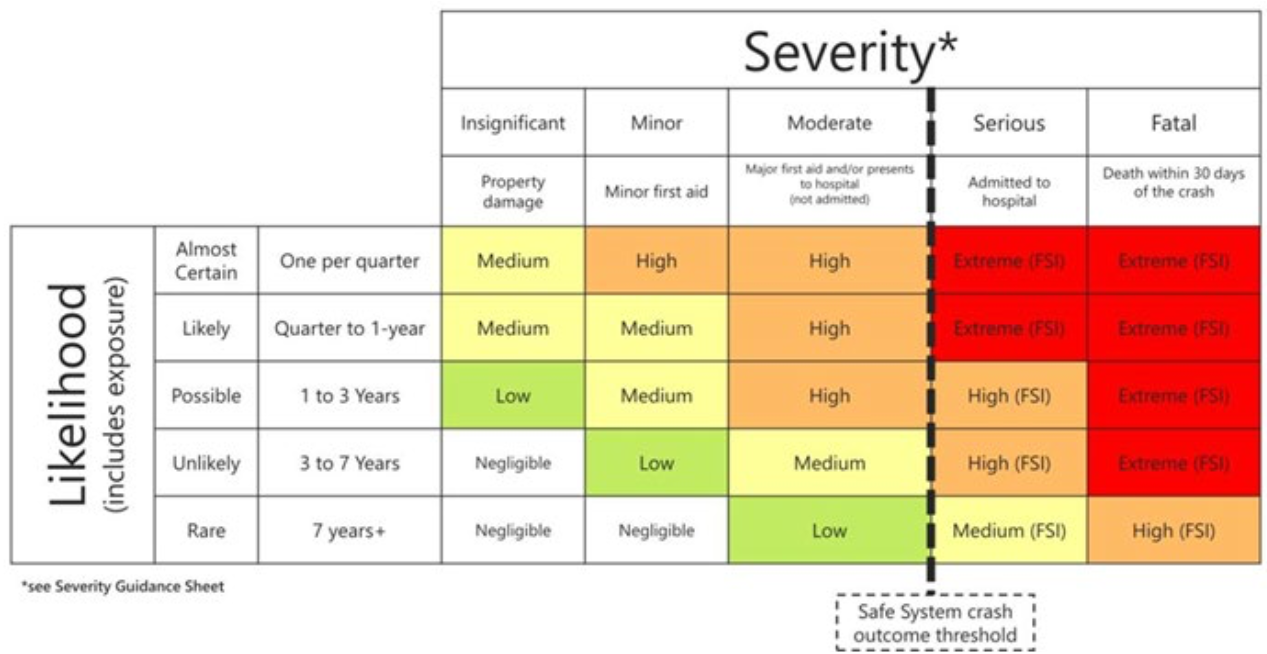
\includegraphics{Austroads_risk_matrix}
\caption{Austroads Road Safety Audit risk matrix}
\label{fig:Austroads_risk_matrix}
\end{marginfigure}


The most recent Guide to Road Safety Auditing\cite{Hillier:2022aa} includes a new risk assessment matrix (Figure \ref{fig:Austroads_risk_matrix}). It is similar to most other risk-management approaches, with likelihood and severity combined to given a ranking of risk from negligible (white) to extreme (red). What is different, however, is the large black line separating 'insignificant', 'minor' and 'moderate' crashes from those that are 'serious' or 'fatal' (Figure \ref{fig:Austroads_risk_matrix_excerpt}).  Under the Safe System and Vision Zero the potential for such Fatal or Serious Injury (FSI) outcomes is \textbf{never} considered acceptable, even if such a crash is highly unlikely.  It is \textbf{not} sufficient to reduce the likelihood of FSI crashes. Rather, hazards that might result in a FSI crash must be eliminated entirely, or treated in a way that reduces the severity of outcomes below the FSI threshold.   


\begin{marginfigure}
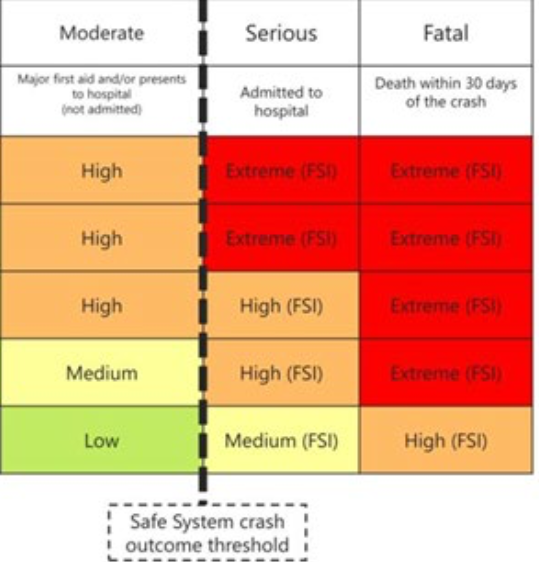
\includegraphics{Austroads_risk_matrix_excerpt}
\caption{Austroads Road Safety Audit risk matrix - Moderate, Serious and Fatal}
\label{fig:Austroads_risk_matrix_excerpt}
\end{marginfigure}


This has resulted in a change to the way that us Road Safety Auditors make findings and recommendations. Under previous approaches auditors might recommend measures that reduce (only)  crash likelihood\footnote{e.g. linemarking, tactile pavement markers or better lighting.}. The problem with this, however, is that when considering the amount of driving done across the population, even if crash likelihood is reduced a thousand-fold, at some stage someone is going to depart the traffic lane\footnote{Or drive towards a low bridge in a high vehicle:\cite{Reynolds:2019aa}} and impact something at speed that might result in death. Measures that reduce crash likelihood still have their place, but the Safe System approach emphasises making even highly unlikely crashes survivable. 

This is part of the reason that wire rope safety barrier, lower speed limits and other such measures that lower crash severity are now often recommended in Road Safety Audits, and more commonly installed along roads. An impact speed of around 70km/hr is the typical threshold for head-on crashes to result in serious injury or fatality\footnote{50km/hr for right angle crashes, 40km/hr for impact with roadside object, 30km/hr for crash involving pedestrian, cyclist or motorcyclist (see Hillier (2022) cited above). That said, a (1-2 ton) car can crush you even moving at low speeds.}. This is why it is now more likely that there will be wire rope safety barrier along the centreline or in the median of freeways or other high-speed environments. Wire rope safety barrier will not reduce the likelihood of an errant vehicle, but it will prevent that vehicle from hitting someone coming in the opposite direction. Hitting the barrier at high speed will still result in a crash. However, unlike a high-speed head-on, hitting a flexible crash barrier first can help to keep impact forces within the range tolerable by humans\cite{TAC:2016aa}.  

\begin{marginfigure}
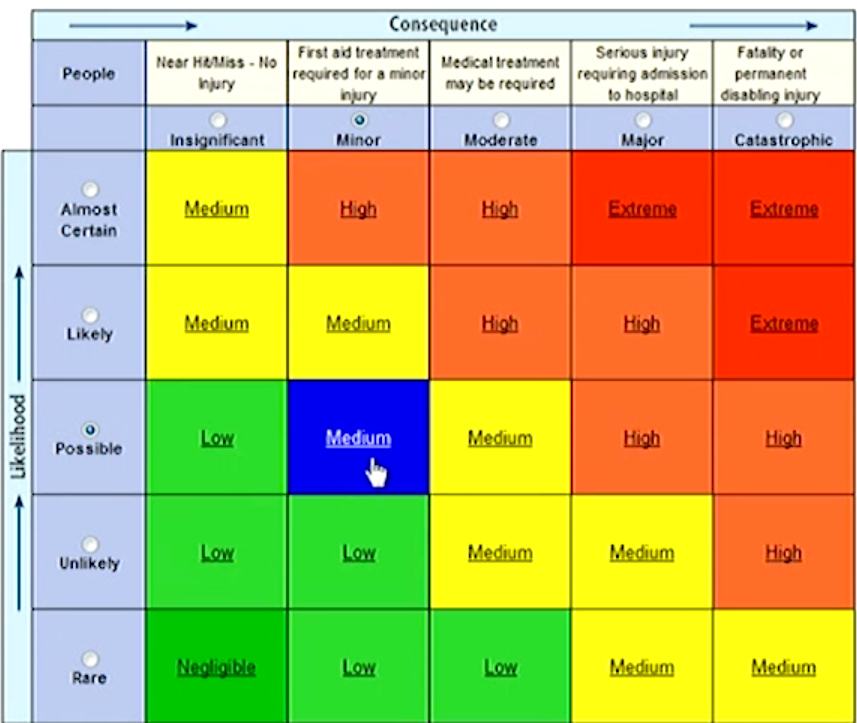
\includegraphics{SARAH_risk_matrix}
\caption{Risk matrix, SARAH}
\label{fig:SARAH}
\end{marginfigure}

\newthought{So what do we do in OH\&S management?} Figure \ref{fig:SARAH} shows the risk matrix used in the SARAH system here at Monash.  The highlighted location is a 'medium' risk, at the intersection of a 'probable' event that results in 'minor' injury (resulting in a need for first aid).  This 'medium' risk level is \textbf{identical} to that for an 'unlikely' event resulting in hospital admission, or a 'rare' event resulting in fatality or permanent disabling injury. Under this risk management approach, all medium risk items might receive the same amount of attention, and further lowering likelihood might be an acceptable way of reducing risk.  Under a 'Vision Zero'-type approach 'medium' risks that have outcomes resulting in hospital admission or fatality (no matter how unlikely) would be separately categorised, identifying a need to reduce consequences below the FSI threshold or eliminate the hazard. 

%\begin{marginfigure}
%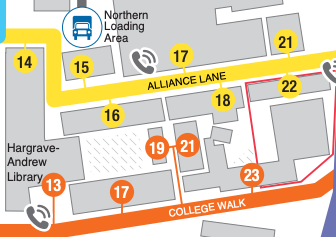
\includegraphics{Clayton_map_excerpt}
%\caption{Alliance Lane and surrounds, Clayton campus}
%\label{fig:Alliance_lane}
%\end{marginfigure}


\begin{marginfigure}
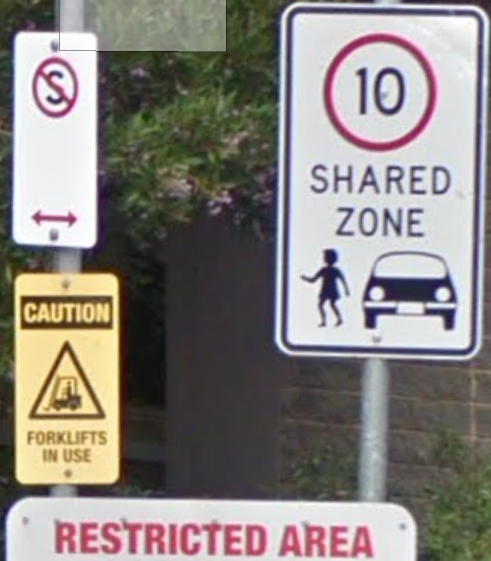
\includegraphics{Alliance_lane_forklifts}
\caption{Alliance Lane warning sign}
\label{fig:Alliance_lane_forklifts}
\end{marginfigure}


Thinking of a practical example from Clayton,  Figure \ref{fig:Alliance_lane_forklifts} shows a warning sign in Alliance Lane, related to forklifts being in use within a shared zone. The purpose of this sign appears to be to reduce the likelihood that a pedestrian and forklift collide, by warning pedestrians to be vigilant. However, pedestrians and forklifts are apparently allowed to both be in Alliance Lane at the same time, meaning that a pedestrian being crushed to death is still a possible (albeit highly unlikely) outcome\footnote{Think of a child that gets away, someone who does not see the sign, or how you may be habituated to ignore the sign because of the countless times you might have walked down Alliance Lane when there were no forklifts active.}. Contrast this to the warehouse space immediately before the checkouts at IKEA. Shoppers and forklifts both use this space, but never together, eliminating the possibility of a collision\footnote{Meanwhile...in the public loading bays outside IKEA...cars and pedestrians everywhere!}. 


\newthought{In summary} the key message from road safety engineering is to focus especially on hazards that might cause serious injury or fatality (no matter how unlikely). Reducing consequences or total elimination of these is at the core of the new(-ish) Vision-Zero-based thinking, although there is clearly a long way to go\footnote{241 road deaths in Victoria in 2022 (Source: https://www.tac.vic.gov.au/)}. While the context in OH\&S is different\footnote{66 workplace deaths in Victoria in 2022 (Source: https://www.worksafe.vic.gov.au)} adopting a Safe-System-informed approach would imply reducing the severity of potentially fatal or serious injury crashes, or to make these entirely impossible, no matter how unlikely they might be. Road safety is shifting to acknowledge that human error is inevitable, and that there is a need to fail safely. I recommend doing the same in your OH\&S risk management.


%\printclassoptions

\nobibliography{safety_day_2023_handout}
\bibliographystyle{plainnat}



\end{document}
